\documentclass[tikz,border=10pt]{standalone}
\usepackage{tikz}
\usepackage{amssymb}
\usetikzlibrary{positioning,shapes.geometric,arrows.meta,fit,calc,backgrounds,shadows}

% Define semantic colors
\definecolor{orchestrator}{RGB}{70,130,180}      % Steel blue
\definecolor{actionserver}{RGB}{60,179,113}      % Medium sea green
\definecolor{planning}{RGB}{186,85,211}          % Medium orchid
\definecolor{hardware}{RGB}{255,140,0}           % Dark orange
\definecolor{accent}{RGB}{220,20,60}             % Crimson

\begin{document}
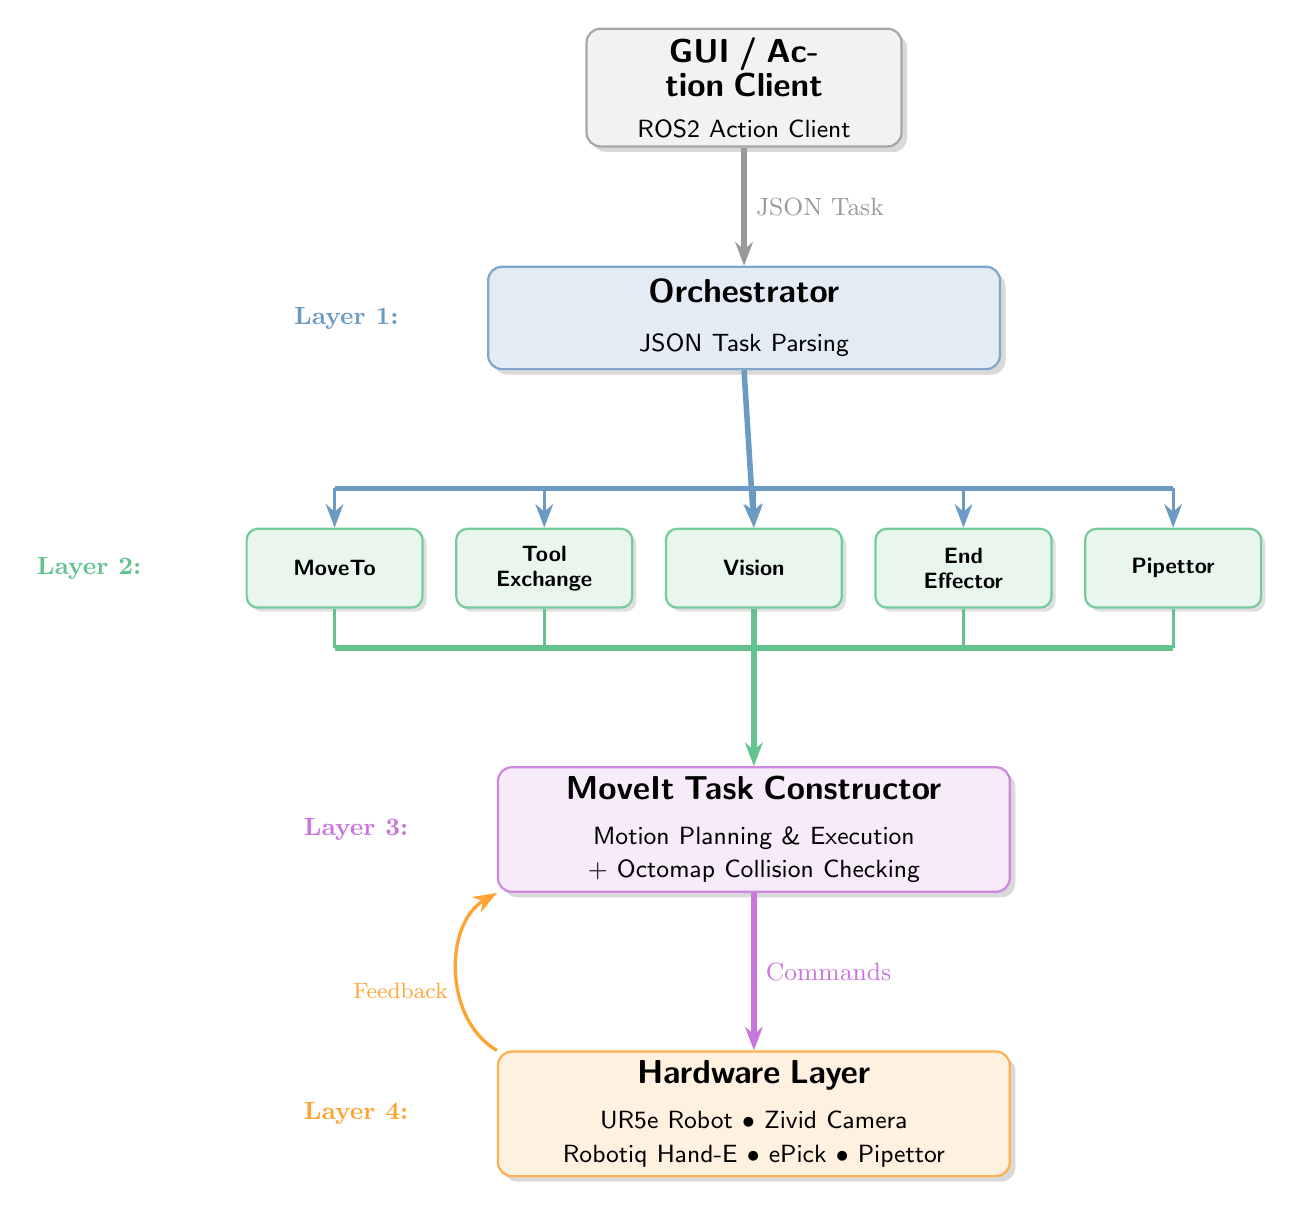
\begin{tikzpicture}[
    node distance=1.8cm,
    font=\sffamily,
    arrow/.style={-{Stealth[length=3mm]}, line width=1.5pt},
    componentbox/.style={
        rectangle,
        rounded corners=5pt,
        minimum width=3.2cm,
        minimum height=1.3cm,
        text centered,
        text width=2.9cm,
        draw,
        thick,
        drop shadow={opacity=0.3, shadow xshift=2pt, shadow yshift=-2pt}
    },
    serverbox/.style={
        rectangle,
        rounded corners=4pt,
        minimum width=2.2cm,
        minimum height=1cm,
        text centered,
        text width=2cm,
        draw,
        thick,
        drop shadow={opacity=0.25, shadow xshift=1.5pt, shadow yshift=-1.5pt}
    }
]

% Title
% \node (title) [font=\LARGE\bfseries, text centered] {EROBS System Architecture};
% \node (subtitle) [below=0.3cm of title, font=\large, text centered, text=gray]
%     {Extensible Robotic Beamline Scientist};

% Layer 0: GUI / Action Client
\node (gui) [
    componentbox,
    draw=gray!70,
    fill=gray!10,
    minimum width=4cm,
    text width=3.7cm
] {
    \textbf{\large GUI / Action Client}\\[0.1cm]
    {\small ROS2 Action Client}
};

% Layer 1: Orchestrator
\node (orchestrator) [
    componentbox,
    below=1.5cm of gui,
    draw=orchestrator!70,
    fill=orchestrator!15,
    minimum width=6.5cm,
    text width=6.2cm
] {
    \textbf{\large Orchestrator}\\[0.2cm]
    {\small JSON Task Parsing }\\
    % {\small Gripper Tracking $\bullet$ Pause/Resume}
};

% Layer 2: Action Servers - 5 in a horizontal line
\node (moveto) [
    serverbox,
    below=2cm of orchestrator,
    xshift=-5.2cm,
    draw=actionserver!70,
    fill=actionserver!12
] {
    \textbf{\footnotesize MoveTo}
};

\node (toolexchange) [
    serverbox,
    right=0.4cm of moveto,
    draw=actionserver!70,
    fill=actionserver!12
] {
    \textbf{\footnotesize Tool}\\[-0.1cm]
    \textbf{\footnotesize Exchange}
};

\node (vision) [
    serverbox,
    right=0.4cm of toolexchange,
    draw=actionserver!70,
    fill=actionserver!12
] {
    \textbf{\footnotesize Vision}
};

\node (endeffector) [
    serverbox,
    right=0.4cm of vision,
    draw=actionserver!70,
    fill=actionserver!12
] {
    \textbf{\footnotesize End}\\[-0.1cm]
    \textbf{\footnotesize Effector}
};

\node (pipettor) [
    serverbox,
    right=0.4cm of endeffector,
    draw=actionserver!70,
    fill=actionserver!12
] {
    \textbf{\footnotesize Pipettor}
};

% Layer 3: MoveIt Task Constructor
\node (mtc) [
    componentbox,
    below=2cm of vision,
    draw=planning!70,
    fill=planning!12,
    minimum width=6.5cm,
    text width=6.2cm
] {
    \textbf{\large MoveIt Task Constructor}\\[0.15cm]
    {\small Motion Planning \& Execution}\\
    {\small + Octomap Collision Checking}
};

% Layer 4: Hardware
\node (hardware) [
    componentbox,
    below=2cm of mtc,
    draw=hardware!70,
    fill=hardware!12,
    minimum width=6.5cm,
    text width=6.2cm
] {
    \textbf{\large Hardware Layer}\\[0.15cm]
    {\small UR5e Robot $\bullet$ Zivid Camera}\\
    {\small Robotiq Hand-E $\bullet$ ePick $\bullet$ Pipettor}
};

% Arrow from GUI to Orchestrator
\draw [arrow, gray!80, line width=2pt] (gui.south) --
    node[right, font=\small, text=gray!80] {JSON Task}
    (orchestrator.north);

% Single arrow from Orchestrator to Action Servers (center)
\draw [arrow, orchestrator!80, line width=2pt] (orchestrator.south) -- (vision.north);

% Horizontal distribution line at action server level
\coordinate (distrib_left) at ($(moveto.north) + (0, 0.5)$);
\coordinate (distrib_right) at ($(pipettor.north) + (0, 0.5)$);
\draw [orchestrator!80, line width=2pt] (distrib_left) -- (distrib_right);

% Vertical drops to each server
\draw [arrow, orchestrator!80, line width=1.2pt] (moveto.north |- distrib_left) -- (moveto.north);
\draw [arrow, orchestrator!80, line width=1.2pt] (toolexchange.north |- distrib_left) -- (toolexchange.north);
\draw [arrow, orchestrator!80, line width=1.2pt] (vision.north |- distrib_left) -- (vision.north);
\draw [arrow, orchestrator!80, line width=1.2pt] (endeffector.north |- distrib_left) -- (endeffector.north);
\draw [arrow, orchestrator!80, line width=1.2pt] (pipettor.north |- distrib_left) -- (pipettor.north);

% Single arrow from Action Servers to MTC (center)
\draw [arrow, actionserver!80, line width=2pt] (vision.south) -- (mtc.north);

% Horizontal collection line at action server level (bottom)
\coordinate (collect_left) at ($(moveto.south) + (0, -0.5)$);
\coordinate (collect_right) at ($(pipettor.south) + (0, -0.5)$);
\draw [actionserver!80, line width=2pt] (collect_left) -- (collect_right);

% Vertical lines from each server to collection line
\draw [actionserver!80, line width=1.2pt] (moveto.south) -- (moveto.south |- collect_left);
\draw [actionserver!80, line width=1.2pt] (toolexchange.south) -- (toolexchange.south |- collect_left);
\draw [actionserver!80, line width=1.2pt] (vision.south) -- (vision.south |- collect_left);
\draw [actionserver!80, line width=1.2pt] (endeffector.south) -- (endeffector.south |- collect_left);
\draw [actionserver!80, line width=1.2pt] (pipettor.south) -- (pipettor.south |- collect_left);

% Arrow from MTC to Hardware
\draw [arrow, planning!80, line width=2pt] (mtc.south) --
    node[right, font=\small, text=planning!80] {Commands}
    (hardware.north);

% Feedback arrow from Hardware to MTC
\draw [arrow, hardware!80, line width=1.2pt] (hardware.north west) to[out=150, in=210]
    node[left, font=\footnotesize, text=hardware!80, pos=0.4] {Feedback}
    (mtc.south west);

% Layer labels on the left
\node [left=1cm of orchestrator, font=\small\bfseries, text=orchestrator!80, anchor=east]
    {Layer 1:};
\node [left=1cm of moveto, font=\small\bfseries, text=actionserver!80, anchor=east, xshift=-0.2cm]
    {Layer 2:};
\node [left=1cm of mtc, font=\small\bfseries, text=planning!80, anchor=east]
    {Layer 3:};
\node [left=1cm of hardware, font=\small\bfseries, text=hardware!80, anchor=east]
    {Layer 4:};

\end{tikzpicture}
\end{document}
